\documentclass[tikz,border=15pt]{standalone}
\usepackage{amsmath}
\usetikzlibrary{positioning, arrows.meta, fit, calc, backgrounds, shapes.multipart}

\begin{document}
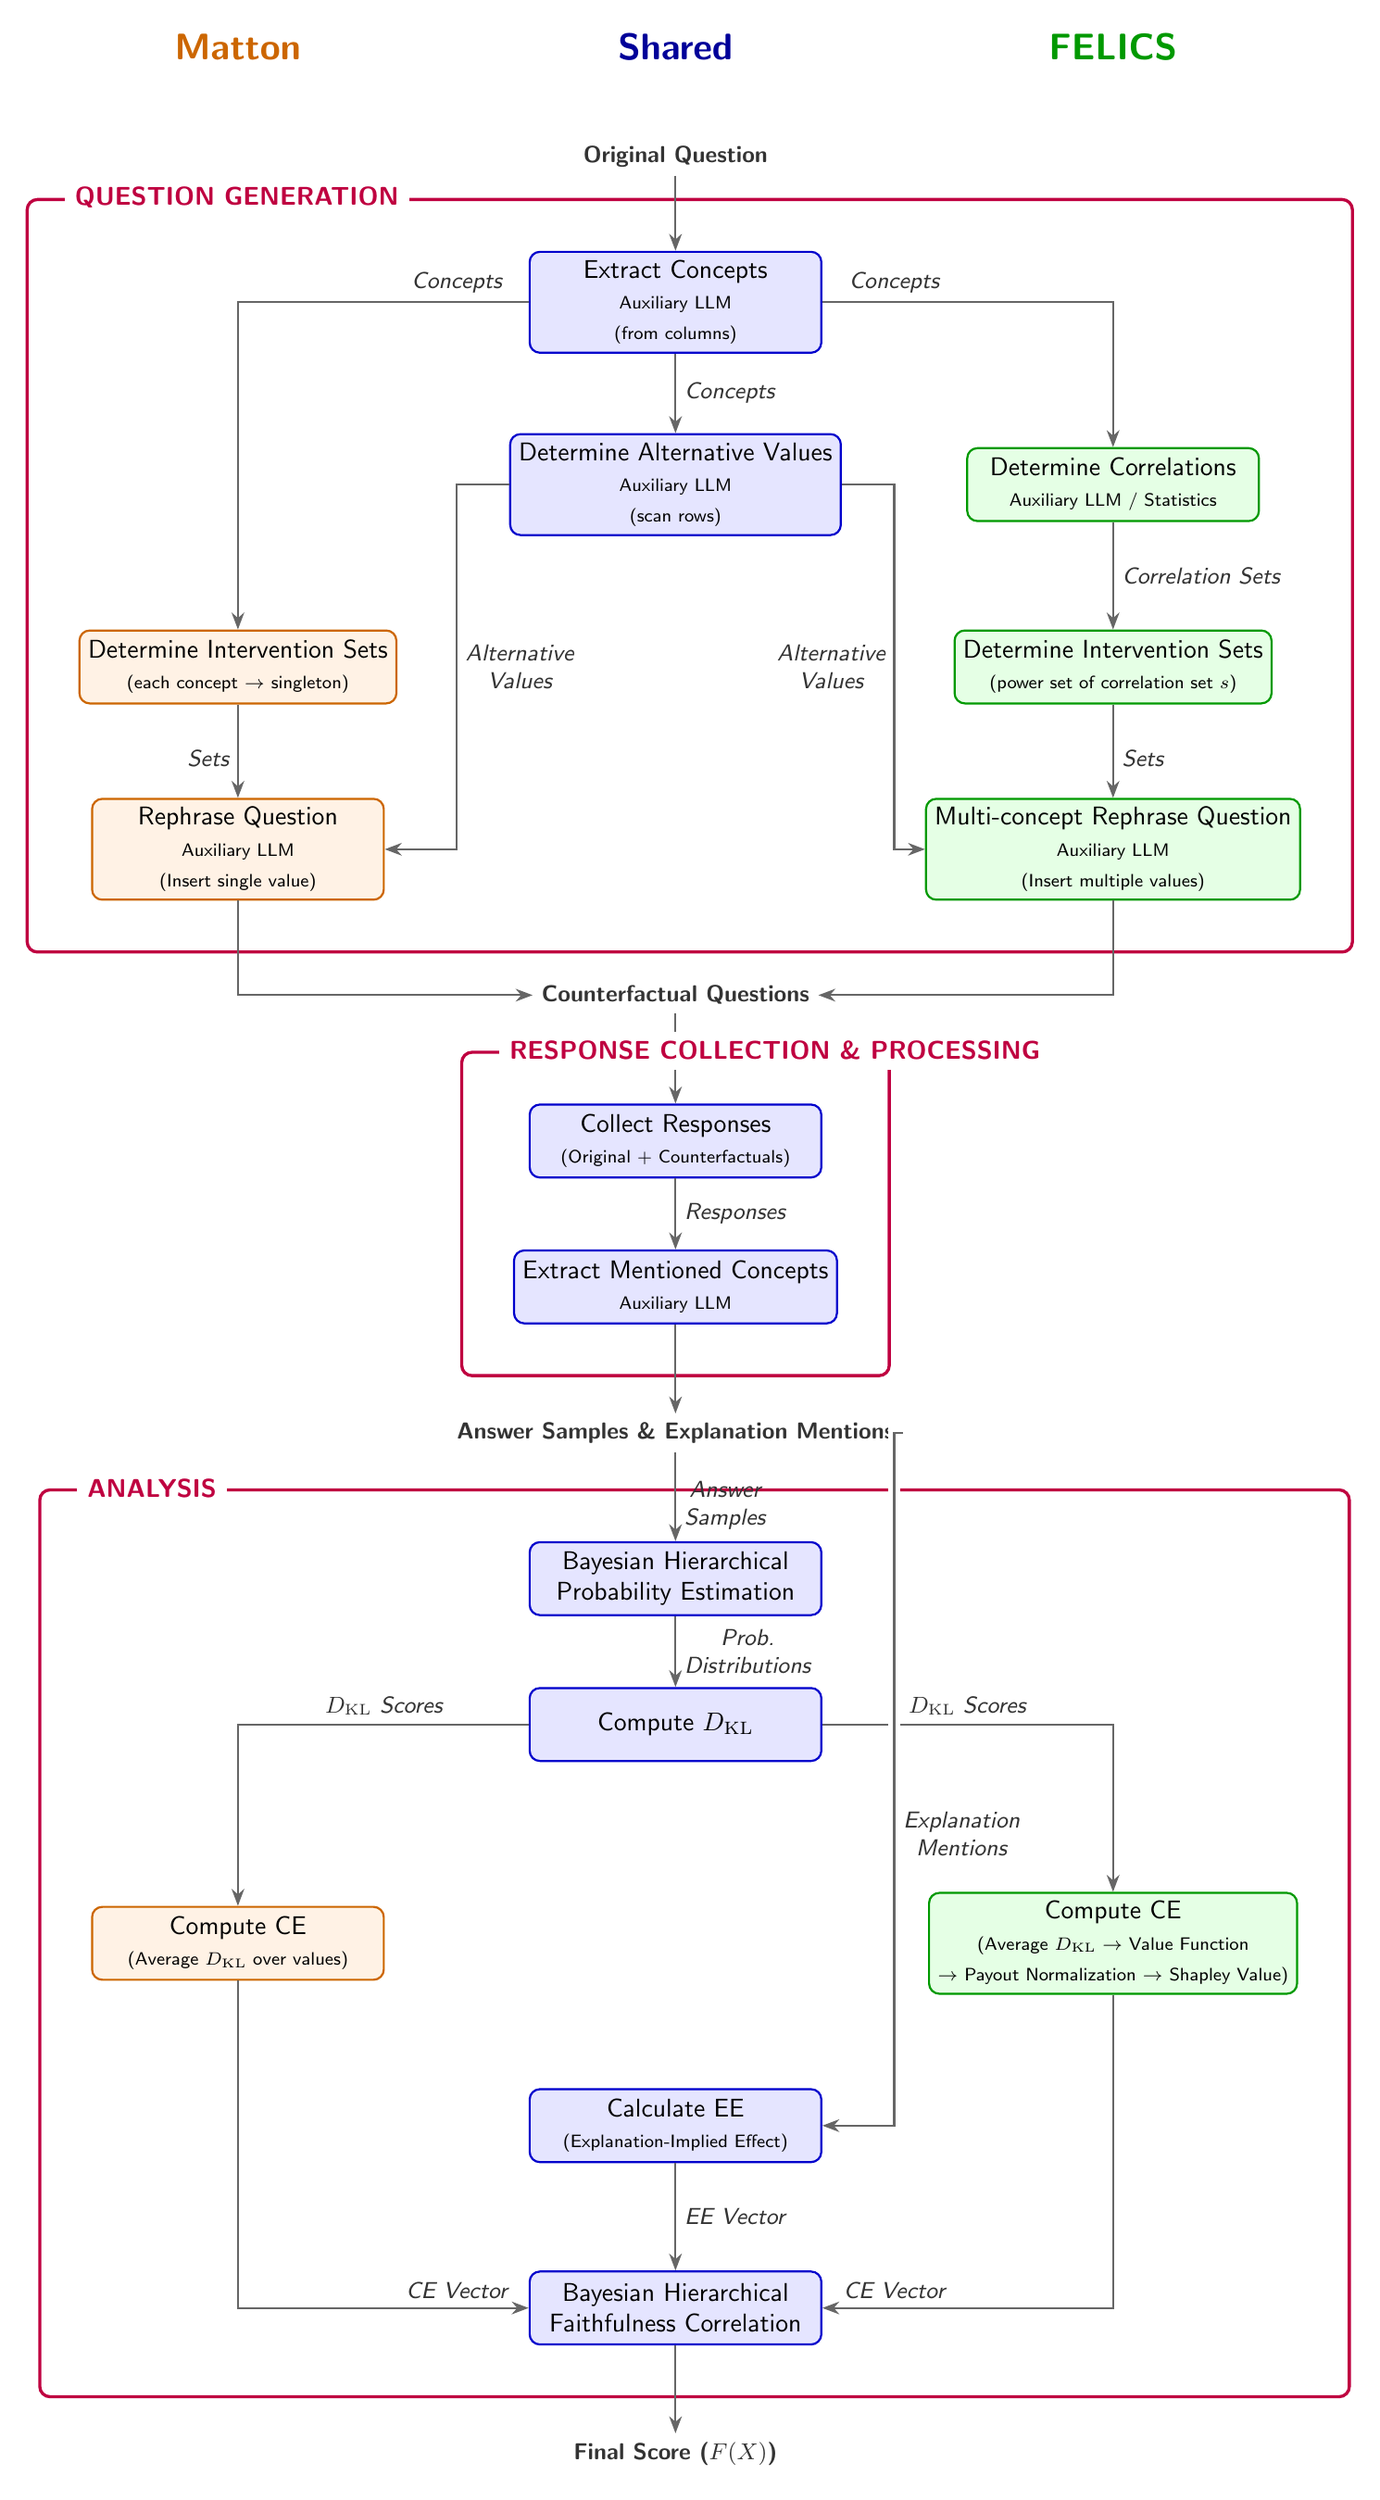
\begin{tikzpicture}[
    node distance=1.5cm and 1.5cm,
    shared/.style={draw=blue!80!black, rounded corners, fill=blue!10, align=center, minimum width=4cm, minimum height=1cm, font=\sffamily, thick},
    matton/.style={draw=orange!80!black, rounded corners, fill=orange!10, align=center, minimum width=4cm, minimum height=1cm, font=\sffamily, thick},
    felics/.style={draw=green!60!black, rounded corners, fill=green!10, align=center, minimum width=4cm, minimum height=1cm, font=\sffamily, thick},
    section/.style={draw=purple, very thick, rounded corners, inner sep=20pt},
    data/.style={font=\sffamily\small\itshape, align=center, color=black!80},
    arrow/.style={->, >=Stealth, thick, draw=gray!80!black},
    crossline/.style={preaction={draw=white, -, line width=5pt}}
]

% ==============================
% GRID AND COLUMNS SETUP
% ==============================
\def\colMatton{-6.0}
\def\colShared{0}
\def\colFelics{6.0}

% Column Headers
\node[font=\sffamily\Large\bfseries\color{orange!80!black}] at (\colMatton, 1.5) {Matton};
\node[font=\sffamily\Large\bfseries\color{blue!60!black}] at (\colShared, 1.5) {Shared};
\node[font=\sffamily\Large\bfseries\color{green!60!black}] at (\colFelics, 1.5) {FELICS};

% ==============================
% TOP INPUT
% ==============================
\node[data] (orig) at (\colShared, 0) {\textbf{Original Question}};

% ==============================
% SECTION 1: QUESTION GENERATION
% ==============================
\node[shared] (extract) at (\colShared, -2) {Extract Concepts\\ \scriptsize Auxiliary LLM\\ \scriptsize (from columns)};
\draw[arrow] (orig) -- (extract);

\node[shared] (altvals) at (\colShared, -4.5) {Determine Alternative Values\\ \scriptsize Auxiliary LLM\\ \scriptsize (scan rows)};
\draw[arrow] (extract) -- (altvals);
\node[data, right] at (\colShared, -3.25) {Concepts};

\node[felics] (correl) at (\colFelics, -4.5) {Determine Correlations\\ \scriptsize Auxiliary LLM / Statistics};
\draw[arrow] (extract.east) -| (correl.north);
\node[data, above] at (3.0, -2) {Concepts};

\node[matton] (matton_set) at (\colMatton, -7) {Determine Intervention Sets\\ \scriptsize (each concept $\rightarrow$ singleton)};
\draw[arrow] (extract.west) -| (matton_set.north);
\node[data, above] at (-3.0, -2) {Concepts};

\node[felics] (felics_set) at (\colFelics, -7) {Determine Intervention Sets\\ \scriptsize (power set of correlation set $s$)};
\draw[arrow] (correl.south) -- (felics_set.north);
\node[data, right] at (\colFelics, -5.75) {Correlation Sets};

\node[matton] (matton_reph) at (\colMatton, -9.5) {Rephrase Question\\ \scriptsize Auxiliary LLM\\ \scriptsize (Insert single value)};
\draw[arrow] (matton_set.south) -- (matton_reph.north);
\node[data, left] at (\colMatton, -8.25) {Sets};
% Safe bus routing for alternative values
\draw[arrow] (altvals.west) -| (-3.0, -9.5) -- (matton_reph.east);
\node[data, right] at (-3.0, -7) {Alternative\\Values};

\node[felics] (felics_reph) at (\colFelics, -9.5) {Multi-concept Rephrase Question\\ \scriptsize Auxiliary LLM\\ \scriptsize (Insert multiple values)};
\draw[arrow] (felics_set.south) -- (felics_reph.north);
\node[data, right] at (\colFelics, -8.25) {Sets};
% Safe bus routing for alternative values
\draw[arrow] (altvals.east) -| (3.0, -9.5) -- (felics_reph.west);
\node[data, left] at (3.0, -7) {Alternative\\Values};

\node[data] (cf_quests) at (\colShared, -11.5) {\textbf{Counterfactual Questions}};
\draw[arrow] (matton_reph.south) |- (cf_quests.west);
\draw[arrow] (felics_reph.south) |- (cf_quests.east);

% Boundary for Section 1
\begin{pgfonlayer}{background}
    \node[section, fit=(extract) (correl) (matton_set) (felics_set) (matton_reph) (felics_reph)] (sec1) {};
\end{pgfonlayer}
\node[font=\sffamily\bfseries\color{purple}, fill=white, inner sep=4pt, anchor=west] at ([xshift=15pt]sec1.north west) {QUESTION GENERATION};


% ==============================
% SECTION 2: RESPONSE COLLECTION & PROCESSING
% ==============================
\node[shared] (collect) at (\colShared, -13.5) {Collect Responses\\ \scriptsize (Original + Counterfactuals)};
\draw[arrow] (cf_quests) -- (collect);

\node[shared] (extract_exp) at (\colShared, -15.5) {Extract Mentioned Concepts\\ \scriptsize Auxiliary LLM};
\draw[arrow] (collect) -- (extract_exp);
\node[data, right] at (\colShared, -14.5) {Responses};

\node[data] (samples) at (\colShared, -17.5) {\textbf{Answer Samples \& Explanation Mentions}};
\draw[arrow] (extract_exp) -- (samples);

% Boundary for Section 2
\begin{pgfonlayer}{background}
    \node[section, fit=(collect) (extract_exp)] (sec2) {};
\end{pgfonlayer}
\node[font=\sffamily\bfseries\color{purple}, fill=white, inner sep=4pt, anchor=west] at ([xshift=15pt]sec2.north west) {RESPONSE COLLECTION \& PROCESSING};


% ==============================
% SECTION 3: ANALYSIS
% ==============================
\node[shared] (bayes_prob) at (\colShared, -19.5) {Bayesian Hierarchical\\ Probability Estimation};
\draw[arrow] (samples.south) -- (bayes_prob.north);
\node[data, right] at (\colShared, -18.5) {Answer\\Samples};

\node[shared] (dkl) at (\colShared, -21.5) {Compute $D_{\mathrm{KL}}$};
\draw[arrow] (bayes_prob.south) -- (dkl.north);
\node[data, right] at (\colShared, -20.5) {Prob.\\Distributions};

\node[matton] (matton_ce) at (\colMatton, -24.5) {Compute CE\\ \scriptsize (Average $D_{\mathrm{KL}}$ over values)};
\draw[arrow] (dkl.west) -| (matton_ce.north);
\node[data, above] at (-4.0, -21.5) {$D_{\mathrm{KL}}$ Scores};

\node[felics] (felics_ce) at (\colFelics, -24.5) {Compute CE\\ \scriptsize (Average $D_{\mathrm{KL}} \rightarrow$ Value Function\\ \scriptsize $\rightarrow$ Payout Normalization $\rightarrow$ Shapley Value)};
\draw[arrow] (dkl.east) -| (felics_ce.north);
\node[data, above] at (4.0, -21.5) {$D_{\mathrm{KL}}$ Scores};

\node[shared] (ee_calc) at (\colShared, -27) {Calculate EE\\ \scriptsize (Explanation-Implied Effect)};

% Crossline bus routing for Explanation Mentions to jump horizontally over the DKL pipeline
\draw[arrow, crossline] (samples.east) -| (3.0, -27) -- (ee_calc.east);
\node[data, right] at (3.0, -23) {Explanation\\Mentions};

\node[shared] (bayes_corr) at (\colShared, -29.5) {Bayesian Hierarchical\\ Faithfulness Correlation};
\draw[arrow] (matton_ce.south) |- (bayes_corr.west);
\node[data, above] at (-3.0, -29.5) {CE Vector};

\draw[arrow] (felics_ce.south) |- (bayes_corr.east);
\node[data, above] at (3.0, -29.5) {CE Vector};

\draw[arrow] (ee_calc.south) -- (bayes_corr.north);
\node[data, right] at (\colShared, -28.25) {EE Vector};

\node[data] (final) at (\colShared, -31.5) {\textbf{Final Score ($F(X)$)}};
\draw[arrow] (bayes_corr.south) -- (final.north);

% Boundary for Section 3
\begin{pgfonlayer}{background}
    \node[section, fit=(bayes_prob) (matton_ce) (felics_ce) (bayes_corr) (ee_calc)] (sec3) {};
\end{pgfonlayer}
\node[font=\sffamily\bfseries\color{purple}, fill=white, inner sep=4pt, anchor=west] at ([xshift=15pt]sec3.north west) {ANALYSIS};

\end{tikzpicture}
\end{document}